\section{Results}

Figure~\ref{fig:P} shows the transition operator $P$.

\begin{figure}[h]
\centering
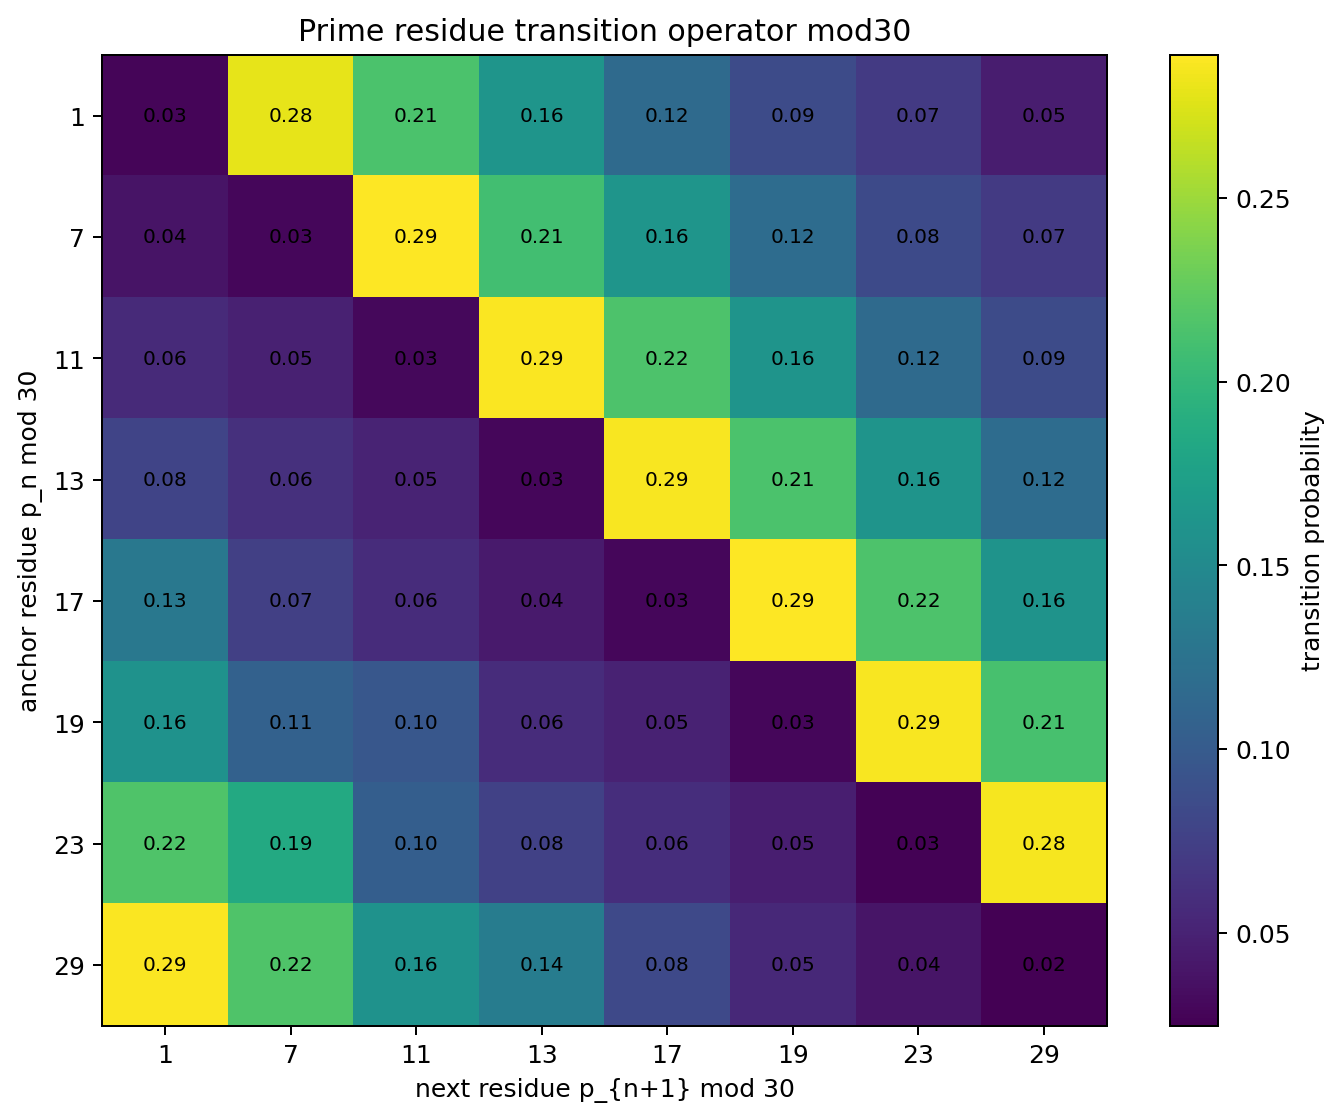
\includegraphics[width=0.6\textwidth]{figures/transition_operator_P_heatmap.png}
\caption{First-order transition operator $P$.}
\label{fig:P}
\end{figure}

Figure~\ref{fig:delta} shows the residual $\Delta = P^{(2)} - P^2$, with nonuniform deviations.

\begin{figure}[h]
\centering
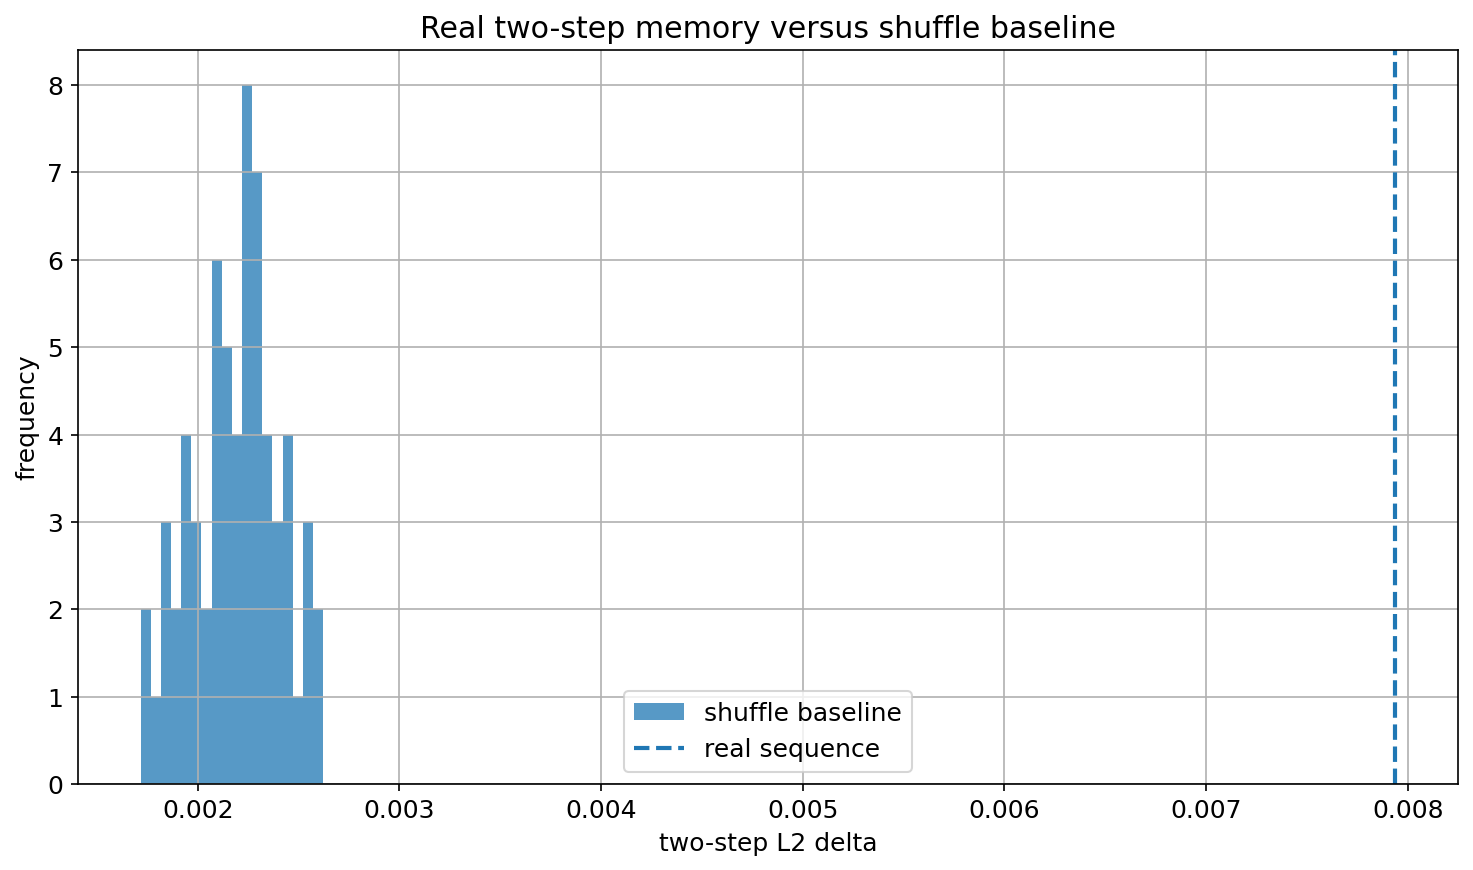
\includegraphics[width=0.6\textwidth]{figures/two_step_delta_heatmap.png}
\caption{Residual operator $\Delta = P^{(2)} - P^2$.}
\label{fig:delta}
\end{figure}

Figure~\ref{fig:lowrank} shows low-rank structure in $\Delta$.

\begin{figure}[h]
\centering
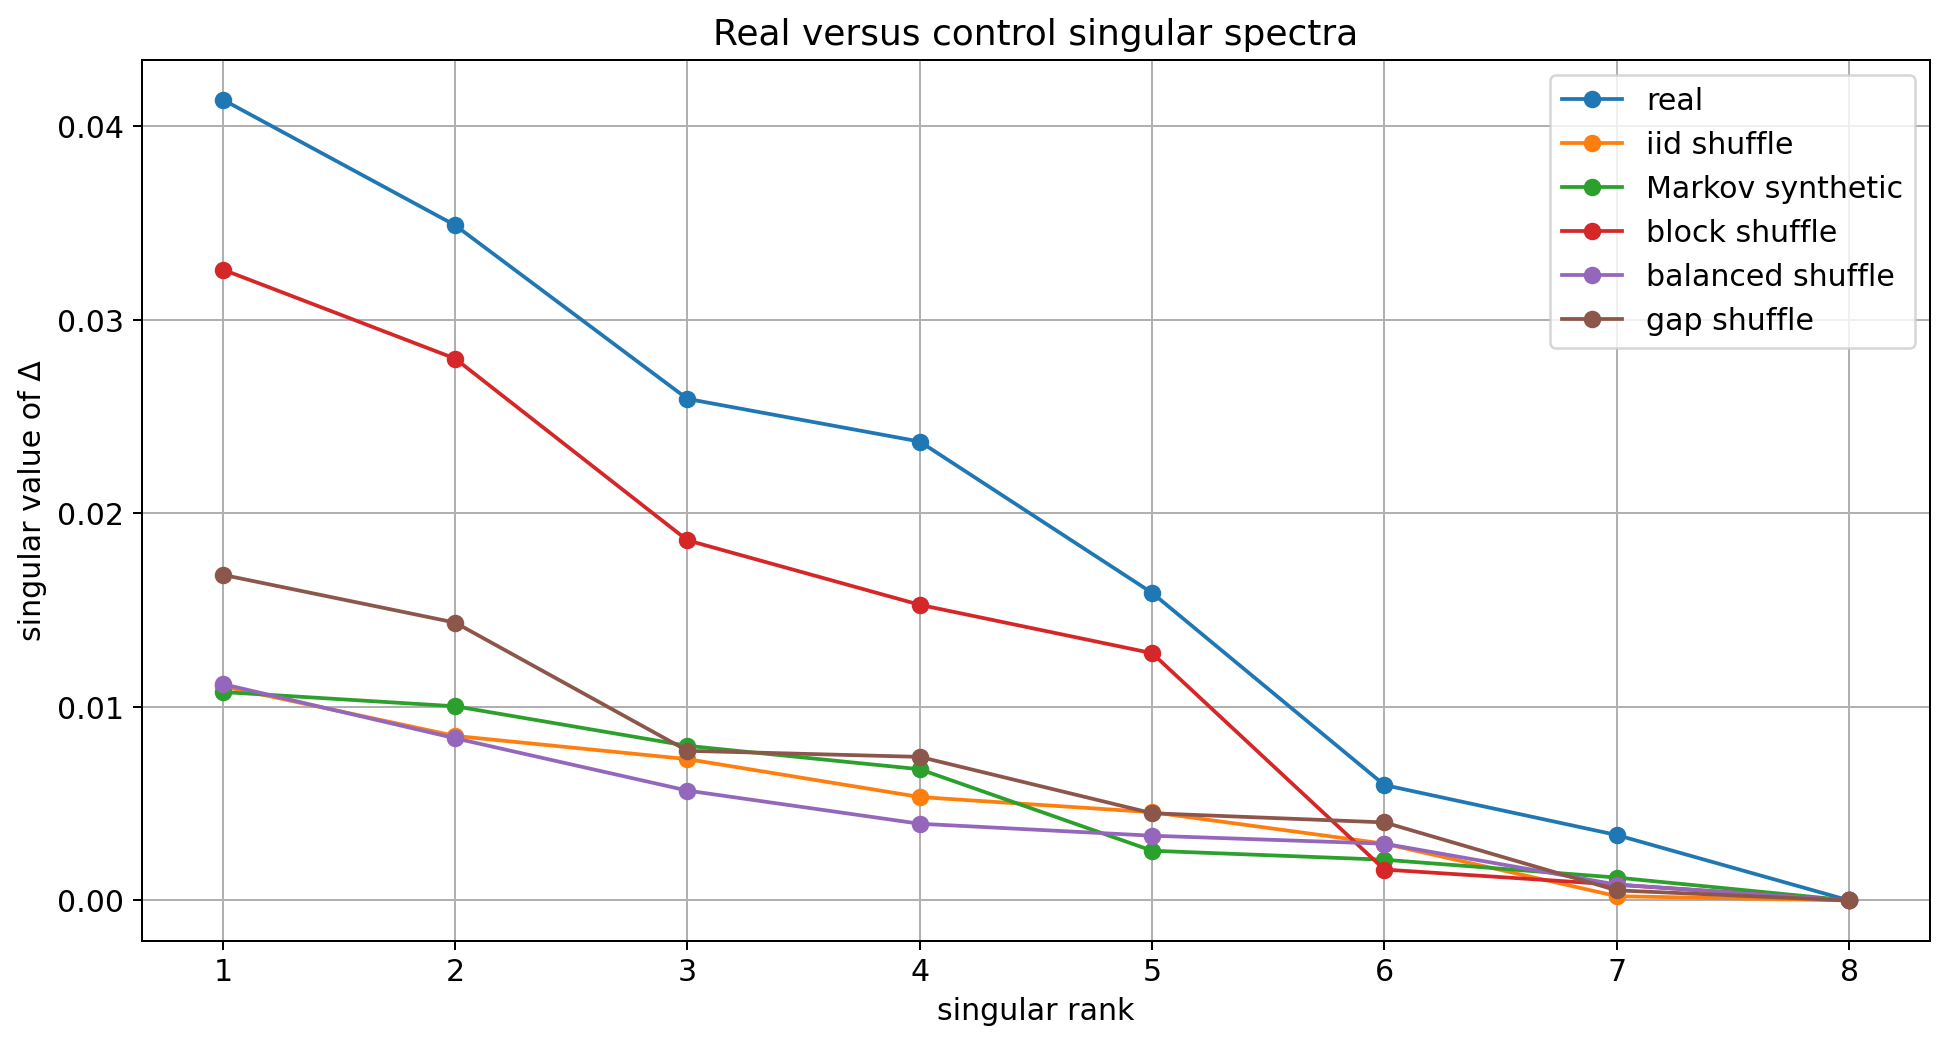
\includegraphics[width=0.6\textwidth]{figures/singular_spectrum_real_vs_null.png}
\caption{Low-rank structure of $\Delta$.}
\label{fig:lowrank}
\end{figure}

Figure~\ref{fig:pvalues} shows statistical validation across controls.

\begin{figure}[h]
\centering
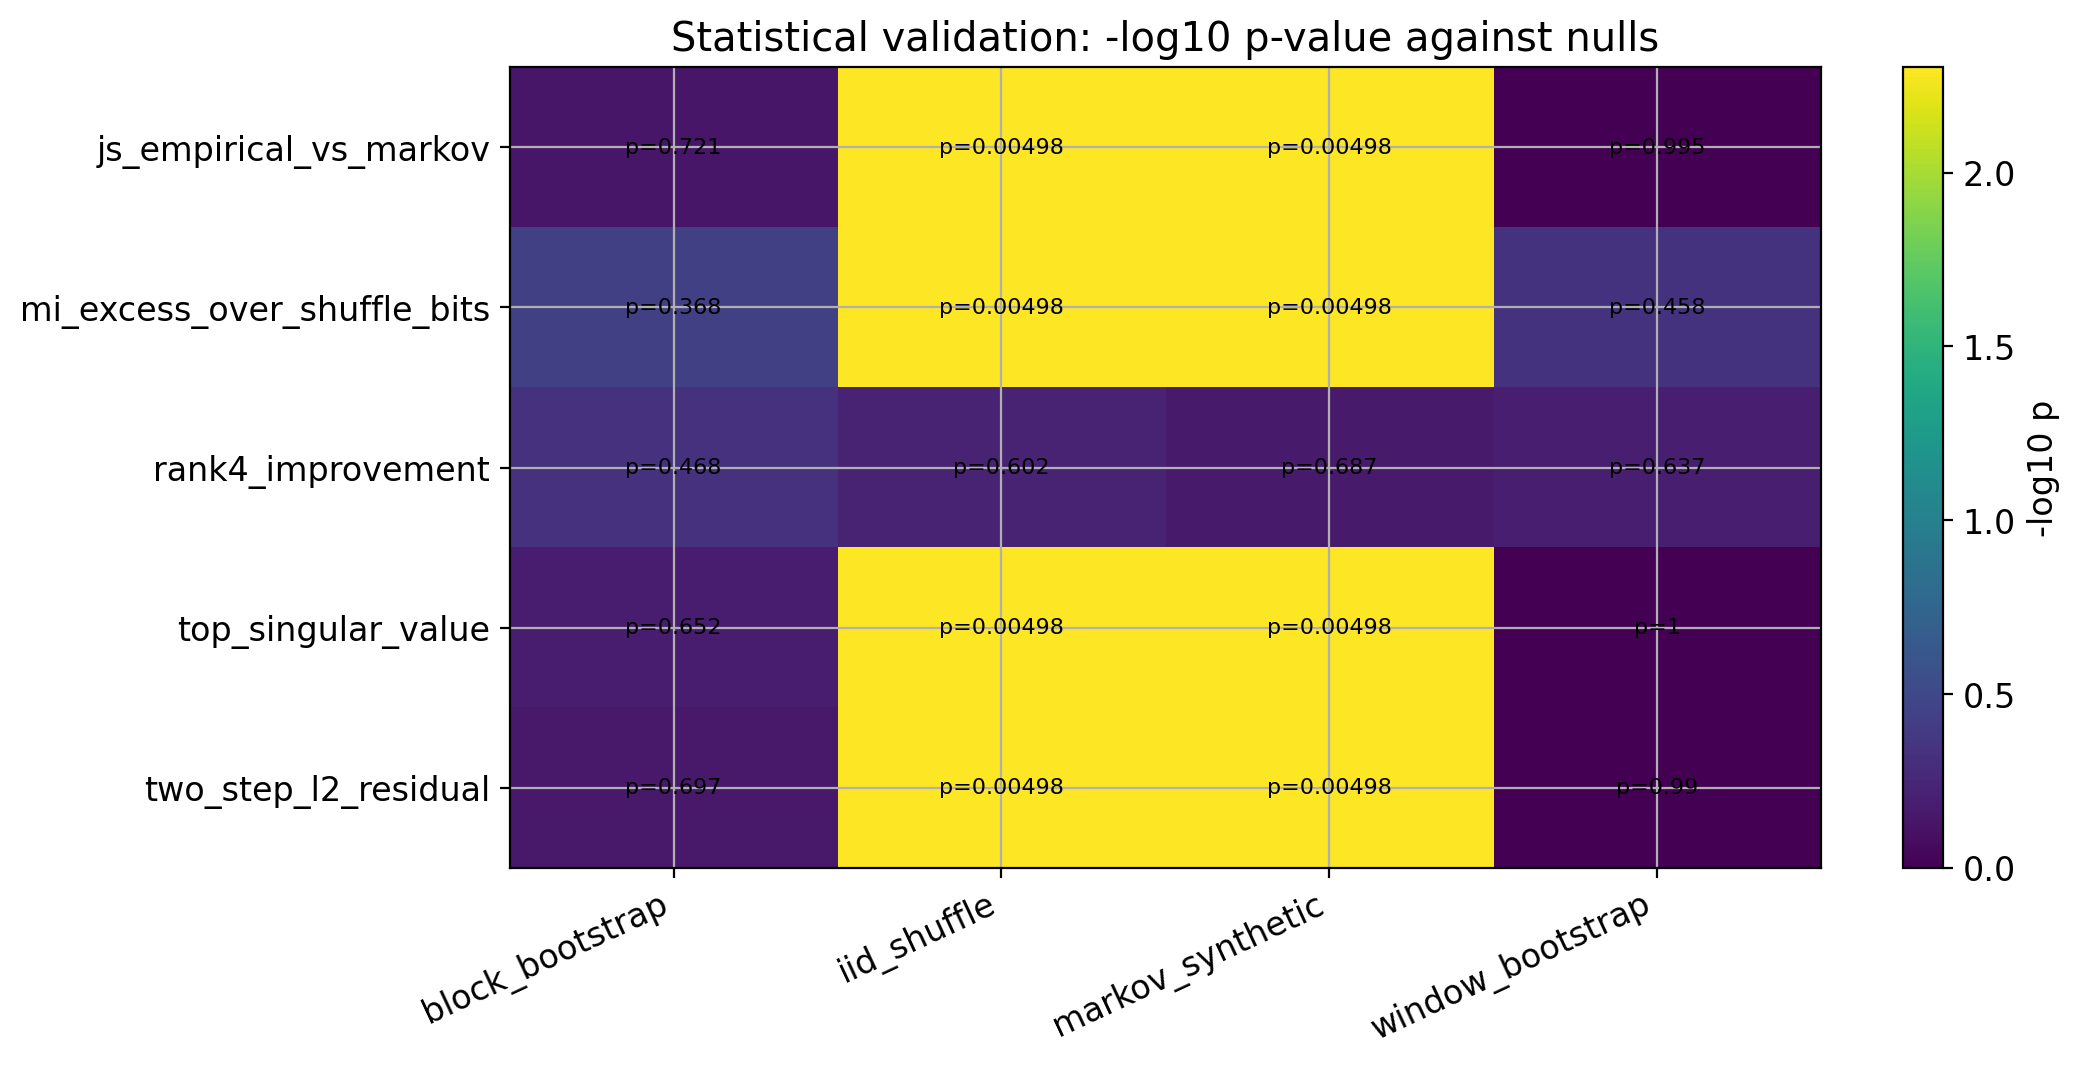
\includegraphics[width=0.6\textwidth]{figures/stat_validation_pvalues.png}
\caption{Statistical validation p-values.}
\label{fig:pvalues}
\end{figure}

Figure~\ref{fig:ratios} shows summary ratios for empirical and control statistics.

\begin{figure}[h]
\centering
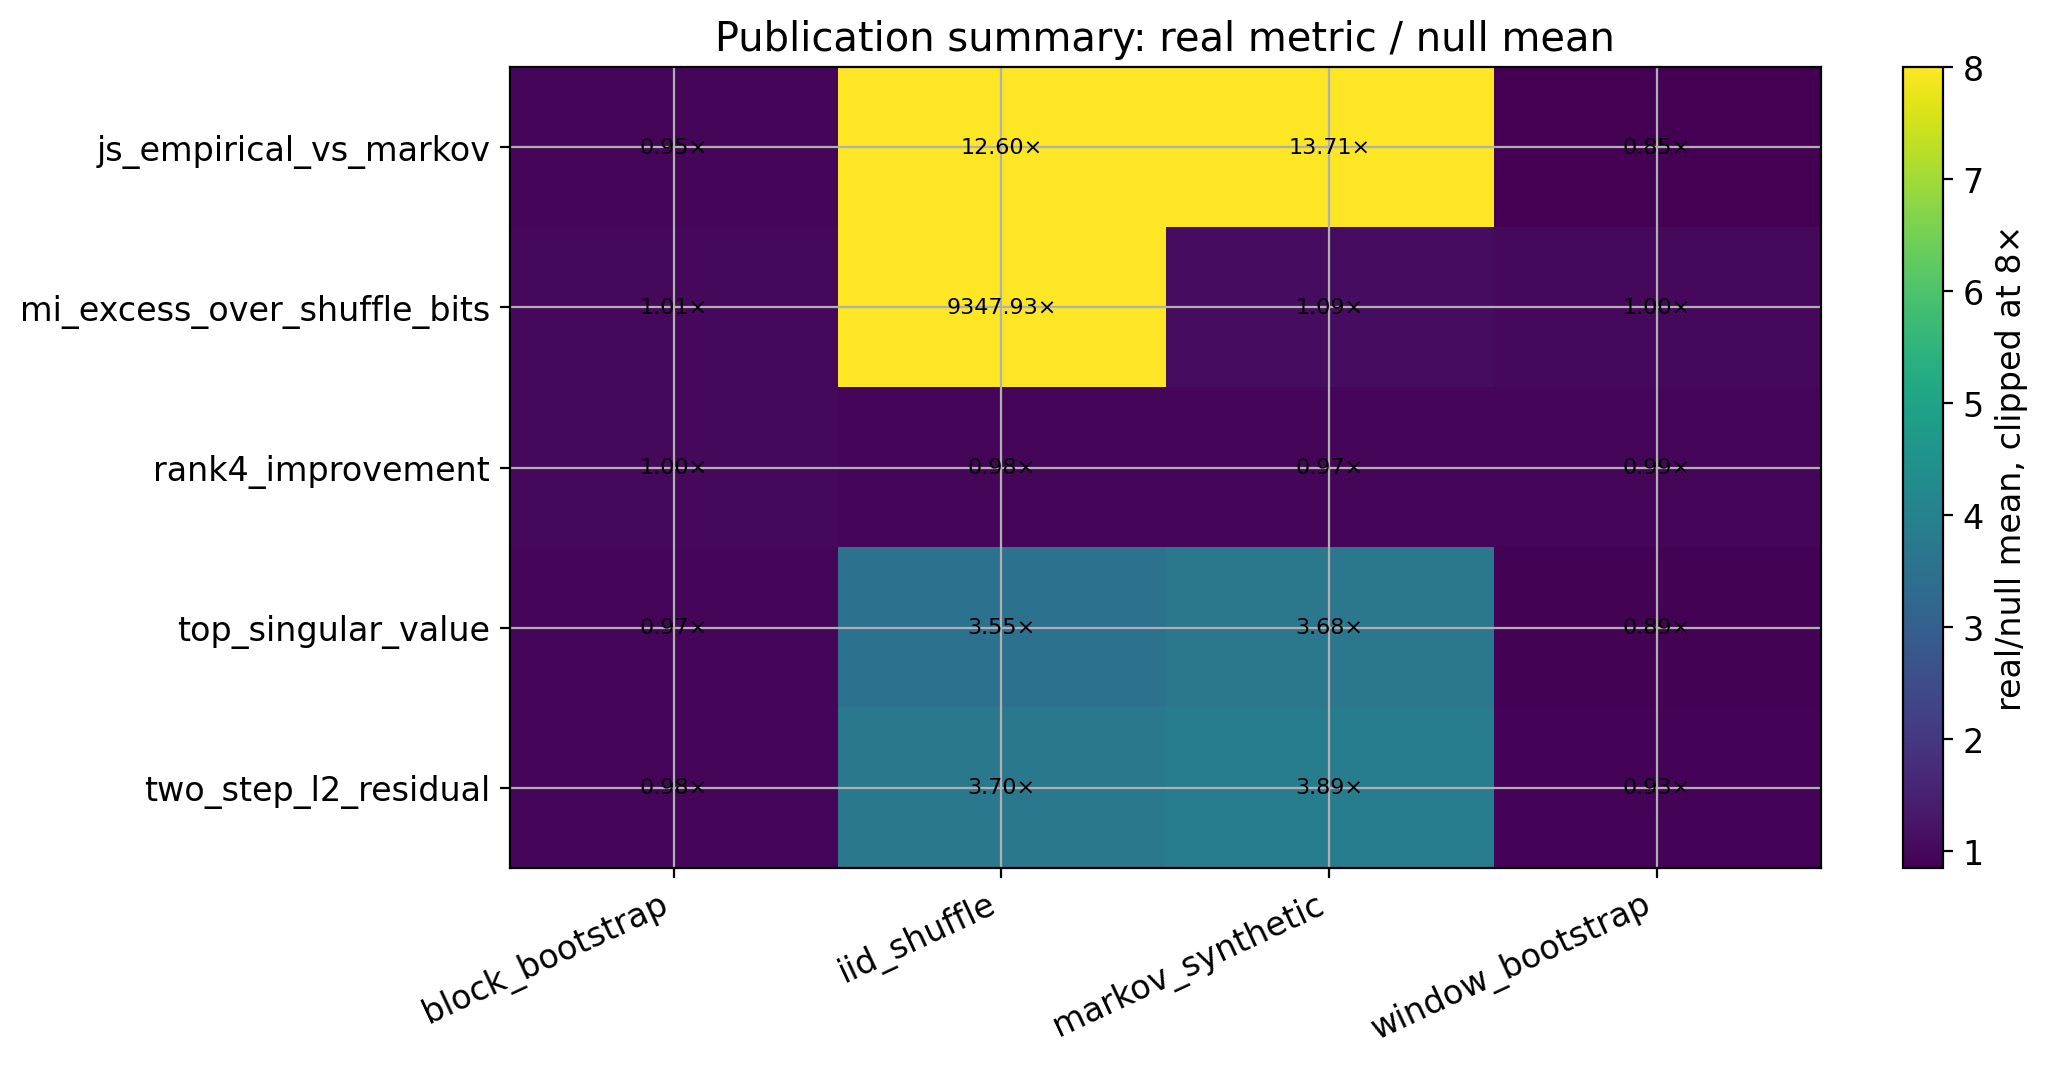
\includegraphics[width=0.6\textwidth]{figures/publication_summary_ratios.png}
\caption{Summary ratios for empirical and control statistics.}
\label{fig:ratios}
\end{figure}
